\documentclass[12pt]{article}
\usepackage{makeidx}
\usepackage[margin=1in]{geometry}  % set the margins to 1in on all sides
\usepackage{graphicx}              % to include figures
\usepackage{amsmath}               % great math stuff
\usepackage{amsfonts}              % for blackboard bold, etc
\usepackage{amsthm}                % better theorem environments
\usepackage{makeidx}               % index
\usepackage[utf8]{inputenc}        % now we have tildes!
\usepackage{wrapfig}               % images
\usepackage{listings}              % Unordered lists

% various theorems, numbered by section

\makeindex



\newtheorem{thm}{Theorem}[section]
\newtheorem{lem}[thm]{Lemma}
\newtheorem{prop}[thm]{Proposition}
\newtheorem{cor}[thm]{Corollary}
\newtheorem{conj}[thm]{Conjecture}

\graphicspath{{maps/}}

\lstset{numberstyle=\scriptsize\ttfamily, numbersep=7pt, captionpos=b}
\lstset{basicstyle=\small\ttfamily}
\lstset{framesep=2pt}

\DeclareMathOperator{\id}{id}

\newcommand{\bd}[1]{\mathbf{#1}}  % for bolding symbols
\newcommand{\RR}{\mathbb{R}}      % for Real numbers
\newcommand{\ZZ}{\mathbb{Z}}      % for Integers
\newcommand{\col}[1]{\left[\begin{matrix} #1 \end{matrix} \right]}
\newcommand{\comb}[2]{\binom{#1^2 + #2^2}{#1+#2}}

\makeatletter
\renewcommand\thesection{\@arabic\c@section}
\renewcommand\thesubsection{\@arabic\c@section.\@arabic\c@subsection}
\makeatother

\begin{document}

\begin{titlepage}

\newcommand{\HRule}{\rule{\linewidth}{0.5mm}} % Defines a new command for the horizontal lines, change thickness here

\center % Center everything on the page

%----------------------------------------------------------------------------------------
%	HEADING SECTIONS
%----------------------------------------------------------------------------------------

\textsc{\LARGE Universidad Carlos III de Madrid}\\[1.5cm] % Name of your university/college
\textsc{\Large Aprendizaje Automático}\\[0.5cm] % Major heading such as course name
\textsc{\large Computer Science Engineering}\\[0.5cm] % Minor heading such as course title

%----------------------------------------------------------------------------------------
%	TITLE SECTION
%----------------------------------------------------------------------------------------

\HRule \\[0.4cm]
{ \huge \bfseries Práctica 1: Clasificación y Predicción}\\[0.4cm] % Title of your document
\HRule \\[1.5cm]

%----------------------------------------------------------------------------------------
%	AUTHOR SECTION
%----------------------------------------------------------------------------------------


% If you don't want a supervisor, uncomment the two lines below and remove the section above
\emph{Authors:}\\
Daniel \textsc{Medina García}\\ % Your name
Alejandro \textsc{Rodríguez Salamanca}\\[3cm] % Your name

%----------------------------------------------------------------------------------------
%	DATE SECTION
%----------------------------------------------------------------------------------------

{\large \today}\\[3cm] % Date, change the \today to a set date if you want to be precise

%----------------------------------------------------------------------------------------
%	LOGO SECTION
%----------------------------------------------------------------------------------------

%
\includegraphics{Logo}\\[1cm] % Include a department/university logo - this will require the graphicx package

%----------------------------------------------------------------------------------------

\vfill % Fill the rest of the page with whitespace

\end{titlepage}

\tableofcontents

\newpage
\section*{Introducción}

\huge Abstract \small

\newpage
\section{Fase 1}

% TODO: revisar en función de los datos que finalmente utilicemos
Para extraer los datos del juego, se partió la función utilizada en el tutorial anterior. Esa base fue ampliada con experimentación, añadiendo y quitando atributos según mejoraba o empeoraba el éxito de clasificación del árbol resultante con distintos algoritmos, según explicaremos en la \emph{Fase 2}.

La inclusión de datos futuros en las líneas del fichero ha sido implementada siguiendo un método de escritura retardada. Así, no se escribe una nueva línea en el fichero hasta que no se conocen todos los datos que se han de escribir, almacenando mientras tanto los datos intermedios. Esto se hizo creando listas globales, que almacenan las líneas incompletas (a falta de datos futuros) en \texttt{future\_lines} y las puntuaciones (para completar las líneas anteriores cuando llegue su turno) en \texttt{future\_score}. Cuando la primera línea esté completa (en este caso, en el sexto turno), se imprimirán en el archivo los datos que ya se tenían junto a los recién llegados, creando así una línea completa.

\newpage
\section{Fase 2}

Explicación de la experimentación tal como se explica en el enunciado. Debe incluir la justificación de los algoritmos seleccionados, de los atributos seleccionados y de cualquier tratamiento sobre los datos que se haya llevado a cabo. Se concluirá con un análisis de los resultados producidos por los algoritmos elegidos y justificación de la elección del modelo final.

En esta fase el equipo dedicó su esfuerzo a realizar tantas pruebas como fuesen posibles, probando diferentes combinaciones de algoritmos, filtros y atributos para generar el modelo basándonos en conocimiento y razonamientos \emph{a priori}.

Para crear un modelo exitoso, hay que tener en cuenta varios factores, a continuación analizaremos cada uno de ellos:

\subsection{Elección de los datos de entrada para la creación del modelo}

Para la elección de la entrada para el algoritmo, partimos de dos bases: los datos de ejecución del agente automático (que, para jugar, se informa tan sólo de los sensores que le indican las distancias a cada uno de los fantasmas) y los de las partidas que jugamos los miembros del equipo, viendo los fantasmas. No es difícil llegar a la conclusión de que el agente humano gana las partidas mucho más rápido que el agente implementado en el \emph{Tutorial 1}, pero eso no tenía por qué indicar que necesariamente los datos del agente de teclado generasen un modelo con un mayor éxito de clasificación. Sin embargo, con posteriores pruebas encontramos un aplastante 10-15\% de diferencia en éxito de clasificación a favor del agente de teclado entre los modelos generados para ambos archivos con \emph{J48} y \emph{BFTree} y evaluados con cross-validation, dos de los algoritmos que conocíamos de tutoriales anteriores y sabíamos generaban árboles bastante buenos. La siguiente tabla ilustra los resultados obtenidos:

\begin{center} 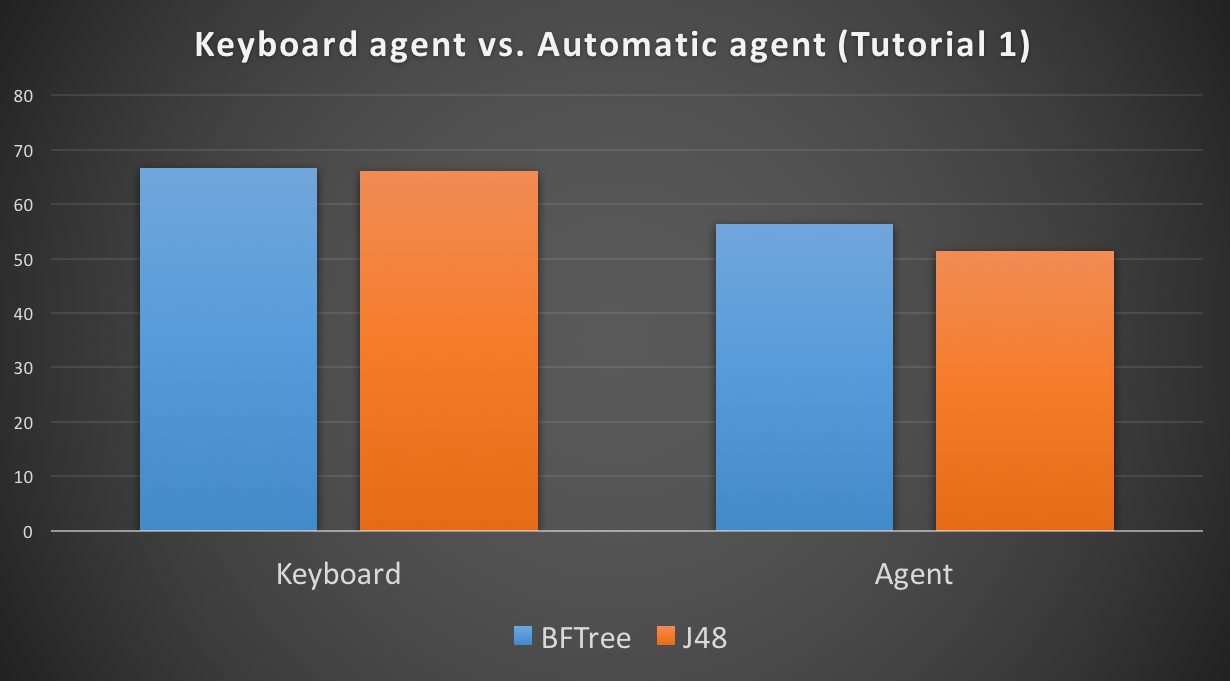
\includegraphics[width=12cm]{kb_vs_aa} \end{center}

Viendo estos datos, nos decantamos por \texttt{training\_keyboard\_edited.arff}, que es el fichero que contiene los datos legales (sin los datos de puntuaciones futuras), para generar el modelo en \emph{Weka}.

\newpage
\subsection{Elección del algoritmo generador de nuestro modelo}

Una vez escogido el archivo que se usará para generar el modelo, comenzamos la comparación entre algoritmos para realizar dicha tarea. Para ello, comparamos varios algoritmos de creación de árboles de decisión evaluándolos tanto con validación cruzada como con dos sets de instancias generadas en partidas jugadas, uno en los mismos mapas que en el entrenamiento y otro en mapas distintos. El éxito de clasificación de cada uno de los algoritmos utilizados se muestra en la siguiente tabla:

\vspace{0.3cm}

\noindent 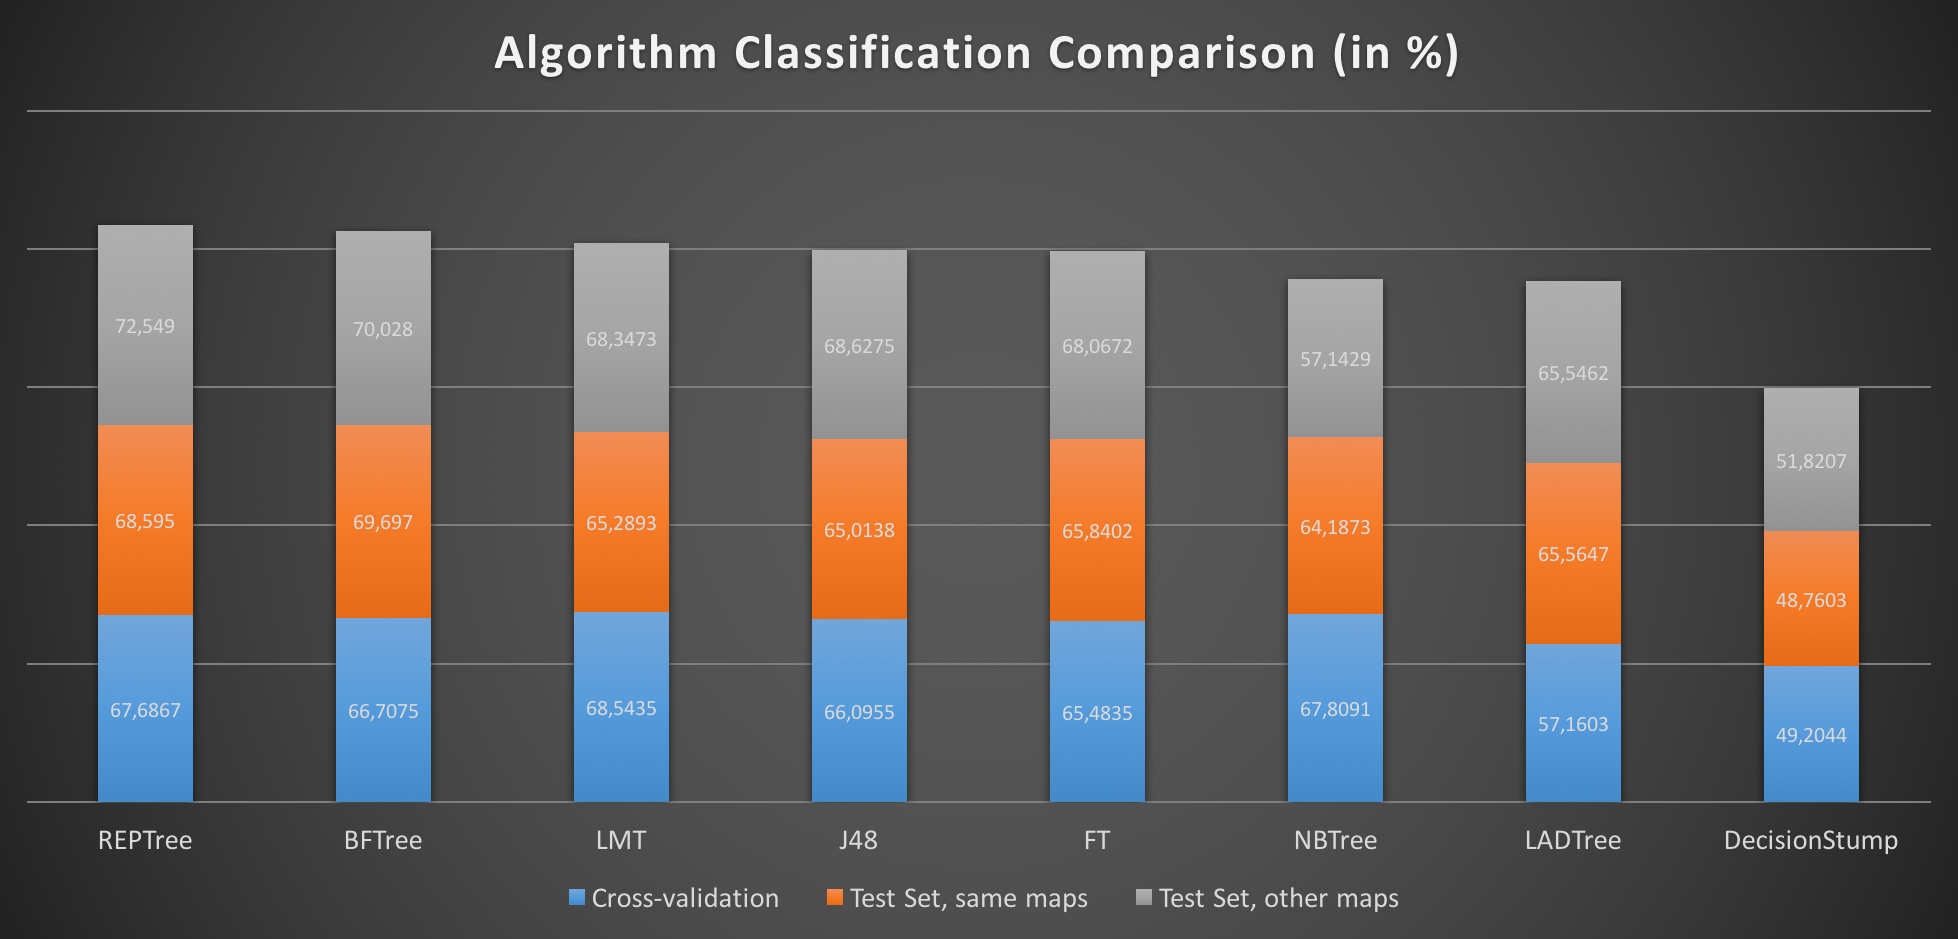
\includegraphics[width=\textwidth]{algorithm_comparison}

\vspace{0.3cm}

Nos sorprendieron los resultados de \emph{REPTree}, un algoritmo que no habíamos utilizado con anterioridad y, sin embargo, obtuvo los mejores resultados. Si bien este algoritmo suele utilizarse para clasificaciones multi-clase, esto no le impide funcionar para una sola clase también, y queda demostrado que con efectividad. Esta información se tendrá muy en cuenta a la hora de elegir el algoritmo generador del modelo en el cual se basará nuestro nuevo agente automático para tomar las decisiones pertinentes, y nos sirve para descartar algunos algoritmos, agilizando los cómputos posteriores.

\subsection{Elección de las modificaciones sobre los datos}

Es este el factor donde el razonamiento sobre los datos puede dar lugar a más variantes. Ya que anteriormente no se han comentado, mencionamos aquí la base de atributos de los que partimos:
\begin{itemize}
    \item \texttt{score} : puntuación actual de PacMan.
    \item \texttt{ghost<N>-living} : True si el fantasma \textless N\textgreater\ sigue vivo, False si ya ha sido comido.
    \item \texttt{distance-ghost<N>} : Distancia ruidosa de PacMan al fantasma \textless N\textgreater.
    \item \texttt{posX} y \texttt{posY} : Coordenadas de PacMan sobre el tablero.
    \item \texttt{direction} : Hacia dónde mira PacMan (último movimiento realizado).
    \item \texttt{wall-<direction>} : True si hay un muro en \textless direction\textgreater, False si vía libre.
    \item \texttt{move} : Movimiento tomado, es la \textbf{clase}.
\end{itemize}

La experimentación ha sido la protagonista, con numerosas pruebas descartadas ante la ausencia de resultados positivos, como son:

\subsection{Creación de nuevos atributos}

Tratamos de agregar los datos que teníamos de forma que resultasen en algún campo que fuese útil para el modelo.

Probamos convirtiendo los atributos \texttt{ghost<N>-living} en uno sólo que fuese la suma de los fantasmas vivos (aplicando primero el filtro \emph{NominalToBinary} sobre los cuatro atributos, y luego el filtro \emph{AddExpression} sumándolos todos), obteniendo un decremento de éxito de entre el 2.3\% y el 3\% dependiendo del método utilizado para la evaluación.

\subsection{Modificación de filtros}

Intentamos extraer el máximo de información de los datos que ya teníamos, sesgándolos mediante la aplicación de filtros que pudiesen acarrear un mejor funcionamiento de los algoritmos de prueba.

Como el movimiento \texttt{STOP} no aporta valor al juego, editamos nuestro fichero de datos eliminando las instancias que hubiesen realizado ese movimiento (i.e. aquellas transcurridas entre que empieza el juego y el jugador de teclado pulsa la primera tecla, ya que era el único momento en el que se producía este hecho) por considerarlas ruidosas. Una vez completada esta primera ``purga'', procedimos a balancear las instancias de cada clase para tener un número similar de instancias que realizasen cada movimiento. Estos fueron los resultados obtenidos en cuanto a éxito de clasificación según los modelos generados:

\vspace{0.3cm}

\noindent 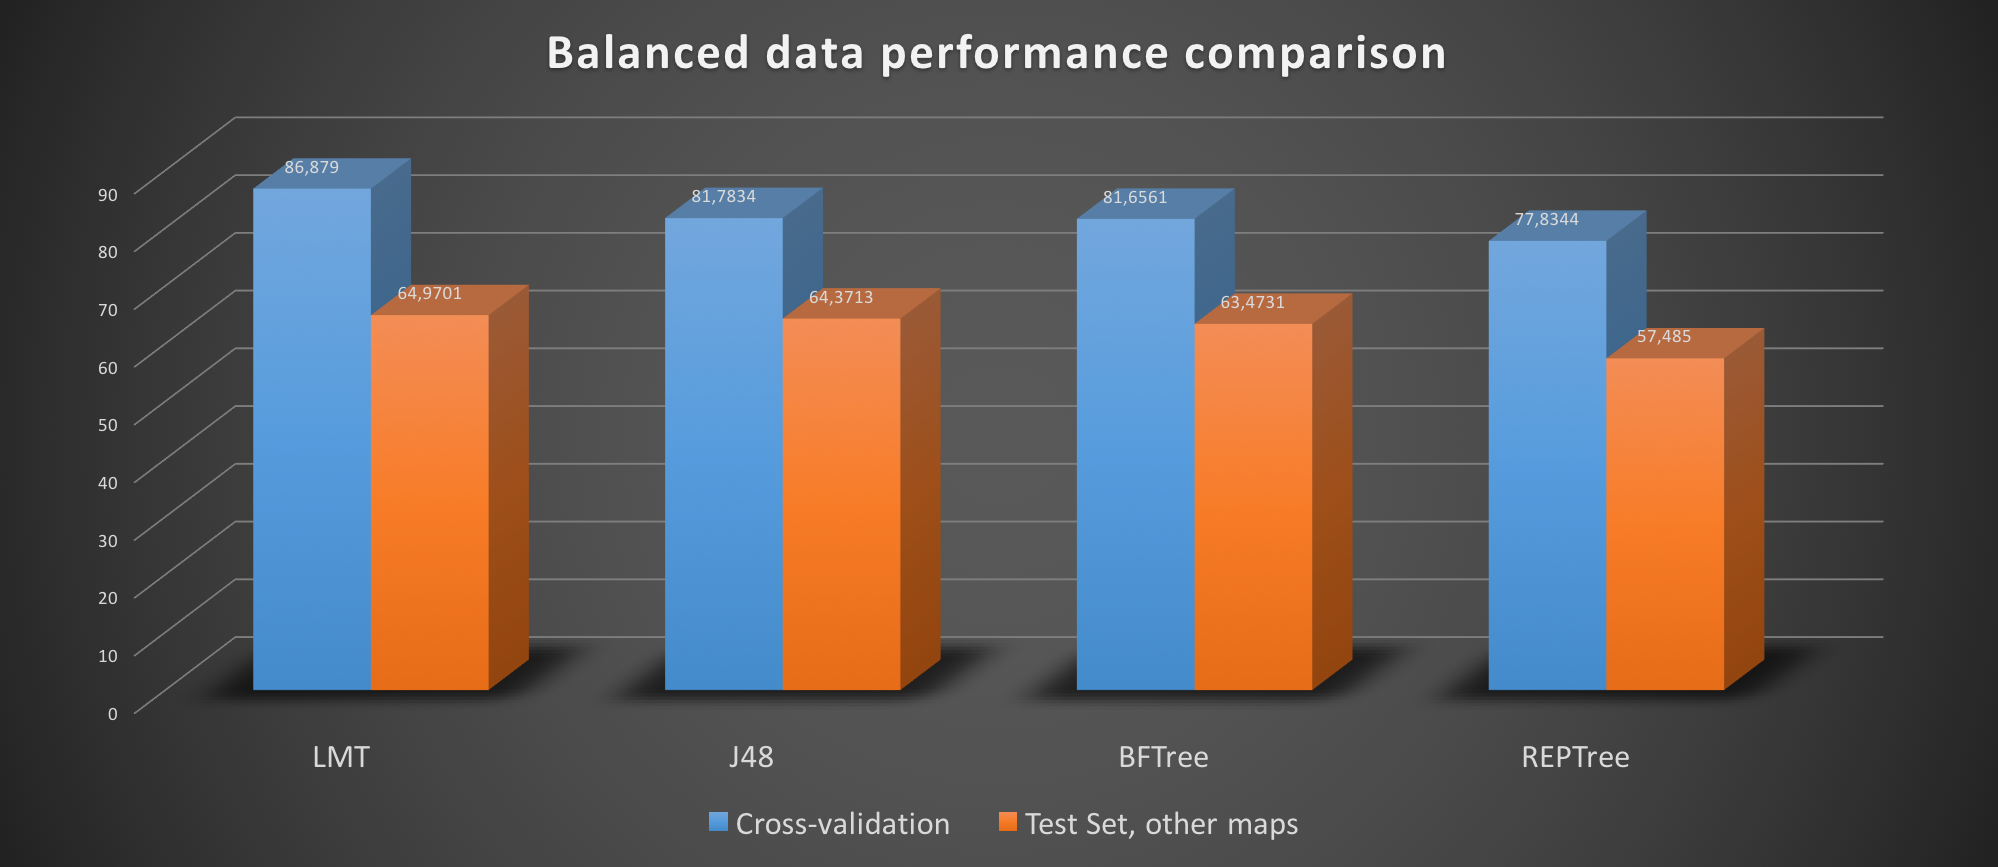
\includegraphics[width=\textwidth]{balanced_performance}

\vspace{0.3cm}

Si bien observamos una clara mejora (de entre el 10 y el 20\%) cuando evaluamos los modelos con validación cruzada, los resultados son desfavorables al evaluar los modelos con una pila de instancias adicional, en otros mapas, decrementando entre un 1 y un 11\% el éxito en clasificación cuando lo comparamos con los datos en bruto.


\newpage
\section{Fase 3}

Igual que en la fase 2, pero con cada modelo de regresión.

\newpage
\section{Preguntas}

\begin{center}
    \vspace{0.5cm} \emph{¿Qué diferencias hay a la hora de aprender esos modelos con instancias provenientes de un agente controlado por un humano y uno automático?}
    \vspace{0.5cm}
\end{center}

Lorem ipsum dolor sit amet, consectetur adipisicing elit, sed do eiusmod tempor incididunt ut labore et dolore magna aliqua. Ut enim ad minim veniam, quis nostrud exercitation ullamco laboris nisi ut aliquip ex ea commodo consequat. Duis aute irure dolor in reprehenderit in voluptate velit esse cillum dolore eu fugiat nulla pariatur. Excepteur sint occaecat cupidatat non proident, sunt in culpa qui officia deserunt mollit anim id est laborum.

\begin{center}
    \vspace{0.5cm} \emph{¿Crees que los resultados del modelo de regresión a 5 turnos vista guardan relación con los de 2 turnos? ¿Por qué?}
    \vspace{0.5cm}
\end{center}

Lorem ipsum dolor sit amet, consectetur adipisicing elit, sed do eiusmod tempor incididunt ut labore et dolore magna aliqua. Ut enim ad minim veniam, quis nostrud exercitation ullamco laboris nisi ut aliquip ex ea commodo consequat. Duis aute irure dolor in reprehenderit in voluptate velit esse cillum dolore eu fugiat nulla pariatur. Excepteur sint occaecat cupidatat non proident, sunt in culpa qui officia deserunt mollit anim id est laborum.

\begin{center}
    \vspace{0.5cm} \emph{Si quisieras transformar la tarea de regresión en clasificación ¿Qué tendrías que hacer? ¿Cuál crees que podría ser la aplicación práctica de predecir la puntuación?}
    \vspace{0.5cm}
\end{center}

Lorem ipsum dolor sit amet, consectetur adipisicing elit, sed do eiusmod tempor incididunt ut labore et dolore magna aliqua. Ut enim ad minim veniam, quis nostrud exercitation ullamco laboris nisi ut aliquip ex ea commodo consequat. Duis aute irure dolor in reprehenderit in voluptate velit esse cillum dolore eu fugiat nulla pariatur. Excepteur sint occaecat cupidatat non proident, sunt in culpa qui officia deserunt mollit anim id est laborum.

\begin{center}
    \vspace{0.5cm} \emph{¿Qué ventajas puede aportar predecir la puntuación respecto a la clasificación de la acción? Justifica tu respuesta.}
    \vspace{0.5cm}
\end{center}

Lorem ipsum dolor sit amet, consectetur adipisicing elit, sed do eiusmod tempor incididunt ut labore et dolore magna aliqua. Ut enim ad minim veniam, quis nostrud exercitation ullamco laboris nisi ut aliquip ex ea commodo consequat. Duis aute irure dolor in reprehenderit in voluptate velit esse cillum dolore eu fugiat nulla pariatur. Excepteur sint occaecat cupidatat non proident, sunt in culpa qui officia deserunt mollit anim id est laborum.

\begin{center}
    \vspace{0.5cm} \emph{¿Crees que se podría conseguir alguna mejora en la clasificación incorporando un atributo que indicase si la puntuación en el instante actual ha descendido o ha bajado?}
    \vspace{0.5cm}
\end{center}

Lorem ipsum dolor sit amet, consectetur adipisicing elit, sed do eiusmod tempor incididunt ut labore et dolore magna aliqua. Ut enim ad minim veniam, quis nostrud exercitation ullamco laboris nisi ut aliquip ex ea commodo consequat. Duis aute irure dolor in reprehenderit in voluptate velit esse cillum dolore eu fugiat nulla pariatur. Excepteur sint occaecat cupidatat non proident, sunt in culpa qui officia deserunt mollit anim id est laborum.

\section{Conclusiones}

Conclusiones técnicas sobre la tarea que se ha realizado.
\begin{itemize}
  \item Apreciaciones más generales como: para qué puede ser útil el modelo obtenido, si al realizar la práctica se os han ocurrido otros dominios en que se pueda aplicar aprendizaje automático, etc.
  \item Descripción de los problemas encontrados a la hora de realizar esta práctica.
  \item Comentarios personales. Opinión acerca de la práctica. Dificultades encontradas, críticas, etc.
\end{itemize}

\end{document}
